\documentclass{article}

\usepackage{amsmath}
\usepackage{amssymb}
\usepackage{tikz}

\begin{document}
\begin{enumerate}
\item [1.8.7.1]
  The pullback lemma states that if both squares of the diagram below are pullbacks then the entire rectangle is a pullback (and vice-versa).
  \begin{center}
    \begin{tikzpicture}
      \node (1) {};
      \node[right of=1,xshift=1cm] (2) {};
      \node[right of=2,xshift=1cm] (3) {};
      \node[below of=1,yshift=-1cm] (4) {};
      \node[right of=4,xshift=1cm] (5) {};
      \node[right of=5,xshift=1cm] (6) {};
      %% Horizontal arrows
      \draw[->] (1) -- (2);
      \draw[->] (2) -- (3);
      \draw[->] (4) -- (5);
      \draw[->] (5) -- (6);
      %% Vertical arrows
      \draw[->] (1) -- (4);
      \draw[->] (3) -- (6);
      \draw[->] (2) -- (5);
    \end{tikzpicture}
  \end{center}

  First, we show that if the squares are pullbacks, the entire rectangle is a pullback.
  That is, we know the following:

  \hfill{}
  \begin{tikzpicture}
    \node (1) {};
    \node[right of=1,xshift=1cm] (2) {};
    \node[below of=1,yshift=-1cm] (4) {};
    \node[right of=4,xshift=1cm] (5) {};
    \node[right of=5,xshift=1cm] (6) {};
    %% Horizontal arrows
    \draw[->] (1) -- node[above]{$f_1$} (2);
    \draw[->] (4) -- node[below] {$f_2$} (5);
    %% Vertical arrows
    \draw[->] (1) -- node[right] {$g_1$} (4);
    \draw[->] (2) -- node[right] {$g_2$} (5);
    %% pullback stuff
    \node[above left of=1,xshift=-1cm,yshift=1cm] (7) {};
    \draw[dashed,->] (7) -- node[above]{$k_1$} (1);
    \draw[->] (7) -- node[above]{$i_1$} (2);
    \draw[->] (7) -- node[left]{$j_1$} (4);  \end{tikzpicture}
  \hfill{}
  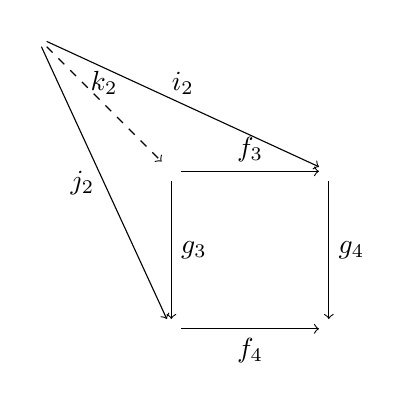
\begin{tikzpicture}
    \node (1) {};
    \node[right of=1,xshift=1cm] (2) {};
    \node[below of=1,yshift=-1cm] (4) {};
    \node[right of=4,xshift=1cm] (5) {};
    %% Horizontal arrows
    \draw[->] (1) -- node[above]{$f_3$}(2);
    \draw[->] (4) -- node[below]{$f_4$}(5);
    %% Vertical arrows
    \draw[->] (1) -- node[right]{$g_3$}(4);
    \draw[->] (2) -- node[right]{$g_4$}(5);
    %% pullback stuff
    \node[above left of=1,xshift=-1cm,yshift=1cm] (7) {};
    \draw[dashed,->] (7) -- node[above]{$k_2$} (1);
    \draw[->] (7) -- node[above]{$i_2$} (2);
    \draw[->] (7) -- node[left]{$j_2$} (4);
  \end{tikzpicture}
  \hfill{}
  
  and want to show that the pair of arrows ($f_1; f_3$), $g$ is a pullback for $(f_2; f_4)$ and $g_1$.

  \begin{center}
    \begin{tikzpicture}
      \node (1) {};
      \node[right of=1,xshift=1cm] (2) {};
      \node[right of=2,xshift=1cm] (3) {};
      \node[below of=1,yshift=-1cm] (4) {};
      \node[right of=4,xshift=1cm] (5) {};
      \node[right of=5,xshift=1cm] (6) {};
      %% Horizontal arrows
      \draw[->] (1) -- node[above] {$f_1; f_3$} (3);
      \draw[->] (4) -- node[below] {$f_2; f_4$} (6);
      %% Vertical arrows
      \draw[->] (1) -- node[right] {$g_1$} (4);
      \draw[->] (3) -- node[right] {$g_4$} (6);
      %% pullback stuff
      \node[above left of=1,xshift=-1cm,yshift=1cm] (7) {};
      \draw[dashed,->] (7) -- node[above]{$k$} (1);
      \draw[->] (7) -- node[above]{$i$} (3);
      \draw[->] (7) -- node[left]{$j$} (4);
    \end{tikzpicture}
  \end{center}

  From the diagram, it is immediately clear that $g_1$ is the pullback arrow for $(f_2; f_4)$.
  The codomain of $g_1$ is the same as the domain of $(f_2; f_4)$, hence for any arrow $j$ that we could replace $g_1$ with and still have a commutative diagram we can map its domain to $\textbf{dom}(g_1)$ using the unique arrow $k_1$.

  The case for $(f_1; f_3)$ is slightly more complicated and I haven't yet finished.
  

\item []
\item [1.8.7.2]
\item []
\item [1.8.7.3]
\item []
\item [1.8.7.4]
\end{enumerate}
\end{document}
